\section{Related Work}\label{sec:relatedwork}
\subsection{Paper folding problem}
Various types of paper crafts have been studied in the field of computation and mathematics. Origami is the Japanese traditional paper art of making different kind of objects by a single sheet of paper, and has been long studied hundreds of years ago\cite{KANADE1980279}.\reply{The simulation of rigid origami is similar to our carton folding problem, while the folding motion is mostly computed based on the given angle of creases, and consider the geometry of origami in kinetic motion~\cite{tachi2009simulation,tachigeometric}. In this paper, cartons are folded into 3D model without knowing the prior of crease angles, and can be deformed through optimization while origami folding cannot deal with the deformation. The thickness problem of origami is also a direction of origami related research these years~\cite{chen2015origami,2016arXiv160105747K,tachi2011rigid}, while thickness is not considered in our problem.}

\reply{Curved folding from a single sheet of paper is a variation of computational origami which considers curved lines as a part of creases, and can be treated as a practical instance of developable surface. Kilian et al.~\cite{Kilian:2008:CF:1360612.1360674} presented an optimization based framework to approximate the given geometric data. Solomon et al.~\cite{Solomon:2012:FDS:2346796.2346817} provided a subdivision based modeling scheme involving curved paper structure with the folding angle on creases as input. Kilian et al.~\cite{Kilian:2017:SAC:3087678.3015460} studied the deformation of curved folded surfaces after the folding motion actuated by pulling a network of string. Despite the 2D expanded layout as an input, curved folding problem always has extra information, such as approximate shape, folding angles or external force, while the carton design layout is our only input.}

While researching on origami in the field of computational algorithm and geometric analysis, the simulation system is developed to visualize the folding behaviour of a single piece of paper. Thiel~\cite{Thiel1998} provides a virtual origami system including the user interface to model folded paper and show animations of folding process. Kishi et al.~\cite{Kishi:1998:OFP:786112.786279} allowed users to create and edit the origami properties over the Web. Nimnual et al.~\cite{Nimnual2007Virtual} presented an application for package folding practices in a virtual space. Although these applications can model folded paper well, they need given parameters to construct the model. How to align constraints to structural designs by implementing shape optimization is our main concern.

There are also some methods to solve related problems of carton folding. 
Song et al.~\cite{Song:2000:MPA:892954} modeled foldable objects as tree like multilink objects and used PRMs~(probabilistic roadmap methods~\cite{Kavraki:1994:PRP:891758}) to find a sequence of motions to transform one configuration of a foldable object into another configuration. 
Mullineux et al.~\cite{Mullineux:2010:CSC:1739328.1739673} provided a simulation framework of the carton during erection using a constraint-based approach. Both these work required the target state as a premise, while our work aim to generate the target configuration.

The complexity of folding to polyhedra problem has also been studied for decades, Lubiw~\cite{Lubiw1996When} provided an dynamic programming algorithm based on Aleksandrov's theorem to test whether a polygon can be folded into polyhedra which takes $O(n^2)$ time and space. 
O'Rourke~\cite{O'Rourke:1998:FUC:646319.686376} examined three open problems on the subject of folding and unfolding. 
Biedl et al.~\cite{Biedl2004When} studied in polynomial time to solve the question of when is the graph orthogonally convex polyhedra given a graph, edge length and facial angles, also shown that it's NP-hard to decide whether the graph is orthogonally polyhedra or not. Rather than the given graph, Biedl et al~\cite{Biedl:2005:NFP:1090462.1646553}. proved that if given a net along with the dihedral angle at each crease, we can know whether a net can be folded to a polyhedron in polynomial time, but it becomes NP-hard without the angles even adding constraints on orthogonal polyhedron, which results in more difficulties on more complex input.
Compared to our desired result, a polyhedron is a set of polygons without overlap, nevertheless, our 3D model contains small faces that needs to be fixed to another panel. 
These works above justify our problem being hard to solve caused by even more intricate inputs.

\subsection{Reconstruction from single line drawings}
\reply{Although with the same goal that constructing 3D models from 2D layouts including vertices and edges as line drawing problem, the construction process is actually different.} 

A line drawing is defined as a 2D projection of object containing its vertexes and edges. Line drawings of three-dimensional objects have long been studied, and the main problem is still in object reconstruction given its projection on two-dimensional planes. 
Some researchers treat this task as an optimization problem. 
Marill~\cite{Marill:1991:EHI:113057.113061} proposed MSDA~(Minimize the Standard Deviation of Angles) principle to emulate the interpretation of line drawings as 3D objects. 
This new criterion is used by many other researchers later. 
Leclerc et al.~\cite{Leclerc1992An} combined MSDA with the deviation from planarity as objective terms. 
Cao et al.~\cite{Cao:2005:ORS:1097114.1097658} added a symmetry measure of the objects to get more complicated results. 
Some other researchers try to solve this problem from the information theoretic point of view. 
Marill~\cite{Marill1992Why} minimized the description length of objects based on the idea that we usually pick the simplest one from infinite possibilities when we see the line drawing. 
Shoji et al.~\cite{Shoji20013} implemented the principle of minimizing the entropy of angle distribution between line segments using genetic algorithm. Later, the strategy of splitting and merging has been used to solve line drawings of complex 3D objects~\cite{10.1109/TPAMI.2010.49,10.1109/CVPR.2014.94}.   
		 
Different from the input above, ours are expanded structural layout of three-dimensional objects in 2D planes, the final model is constructed based on the folding process instead of mathematical presentation.

\begin{figure}
	\centering
	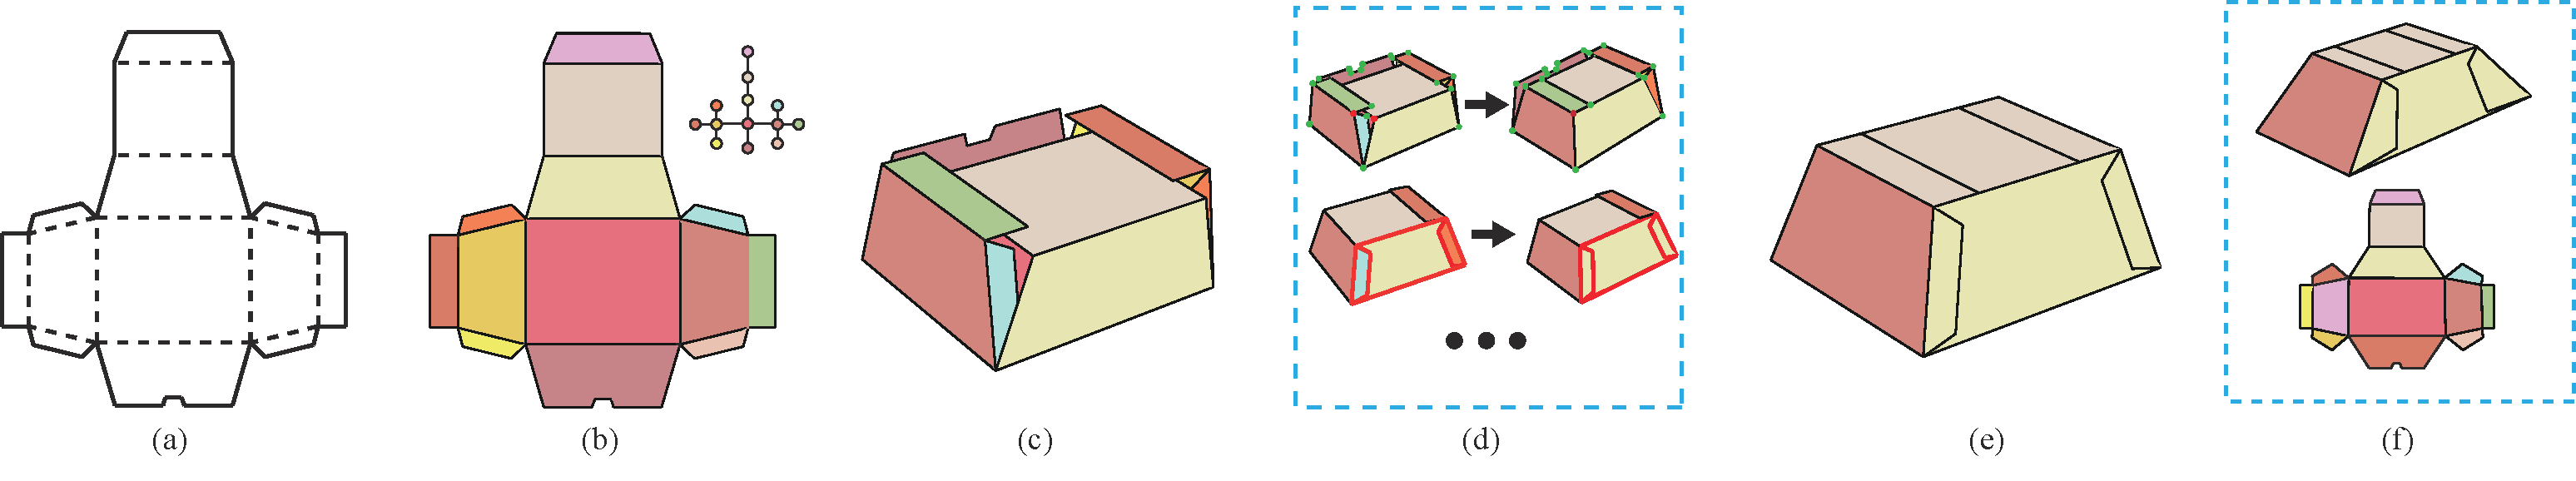
\includegraphics[width=0.9\textwidth]{images/overview}
	\caption{Given a 2D layout (a), we first extract its 2D mesh (b), with different face in different color. By providing each folding edge with a specific angle, we can construct an initial 3D model (c). The final carton model (e) is built through the shape optimization based on the information acquired from user interactions (d).}
	\label{fig:overview}
\end{figure} 

\subsection{Shape optimization}
\reply{The basic idea of our paper is shape optimization by a set of simple algorithms, }
multiple algorithms have been proposed to enforce shape constraints, and have been used successfully for interactive tools and physical simulation~\cite{Botsch:2006:PCP:1281957.1281959,Igarashi:2005:ASM:1186822.1073323}. 
Bouaziz et al.~\cite{Bouaziz:2012:SSD:2346796.2346802} unified a large variety of geometric constraint into one optimization framework, and provided simple, and robust implementation. 
Poranne et al.~\cite{Poranne2013Interactive} described an interactive method to manipulate and optimize polyhedral meshed with constraints with a linear-time algorithm. 
Tang et al.~\cite{Tang:2014:FPM:2601097.2601213} solved constrained equations by Newton-type method in a fast way, and provided an interactive system to model meshed constrained by equalities and inequalities. 
Deng et al.~\cite{Deng2015} developed an interactive tool to explore architectural design with shape constraints, and provided an optimization method to enforce hard constraints and soft constraints at the same time. 

The studies mentioned above focus on the architectural design with constraints, and proposed different solutions, while our constraints do not need satisfy properties like fairness. As a result, we implement the shape optimization by the method introduced in \cite{Bouaziz:2012:SSD:2346796.2346802} for its robustness and simplicity.
%In our paper, we implement the shape optimization by the method introduced in \cite{Bouaziz:2012:SSD:2346796.2346802} for its robustness and simplicity.



